\clearpage
\section{Løsningsdesign}
I dette afsnit er formålet, at finde og beskrive løsningsforslag til den endelige problemformulering. Først er den overordnede ide bag løsningen beskrevet, hvorefter der undersøges hvilken tilgang til udviklingen af løsningsforslaget, som er mest oplagt. Dette gøres ved at se på de teknologier, som kan anvendes til at visualisere en lampe og dens belysning.

\subsection{Ide}

I dette afsnit er der beskrevet en ide til løsningen af den endelige problemformulering. Ideen er resultatet af en diskussion i gruppen, hvor vi kom med ideer til løsninger, og herefter diskuterede fordele og ulemper ved de forskellige ideer. Formålet med afsnittet er at skitsere gruppens bud på den optimale løsning på problemet, og afsnittet er derfor udarbejdet med feedback fra forskellige lampebutikker. I slutningen af afsnittet vil der være en afgrænsning af løsningen som vil danne grundlag for den senere udvikling af en løsning.

Den løsning som gruppen har valgt at arbejde med er, "3D modeller af lamper med interaktion". Som beskrevet i problemanalysen har gruppen valgt at løse problemet når kunder handler på e-butikker. Tanken er derfor at implementere software på en e-butiks hjemmeside med henblik på at løse problemet for kunden.

\subsubsection{Skitse af løsning}

\begin{figure}[H]
   \centering
   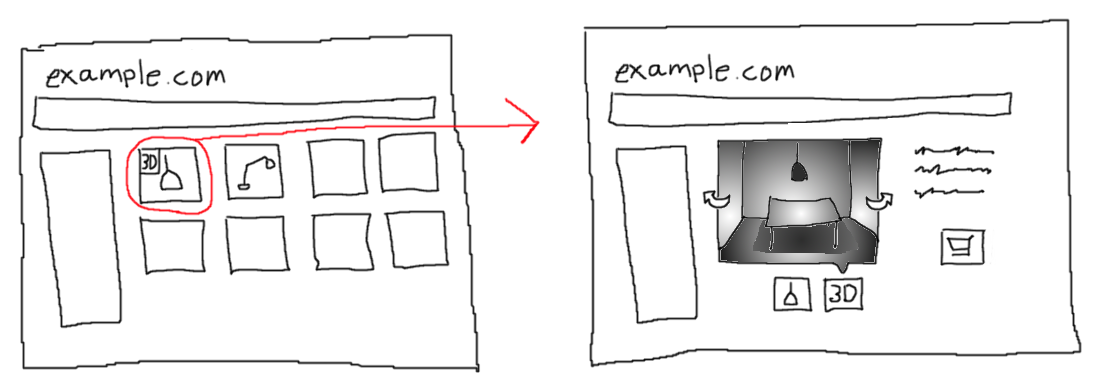
\includegraphics[width=\textwidth]{skitse_til_loesning}
   \caption{Skitse af ide til løsning.}
\end{figure}

På figur 5 er der illusteret en skitse af en e-butik som sælger lamper. Figuren illustrerer hvordan systemet kan integreres på en hjemmeside. Skitse 5a viser et online katalog over e-butikkens udvalg af lamper. Som der fremgår af skitsen vil nogle lamper være markeret med et "3D-ikon" og dette indikerer, at kunden har mulighed for, at se skitsen i 3D. Kunden tilgår 3D-billedet ved at klikke på ikonet. Når kunden trykker på ikonet bliver kunden omdirigeret til en anden menu. Som der fremgår af skitse 5b, så har kunden her mulighed for at se en 3D-model af lampen i et rum. De to pile på skitsen indikerer, at kunden har mulighed for at rotere billedet, og se hvordan belysningen fra lampen er, set fra forskellige vinkler. Som en ekstra feature har kunden mulighed for at indtaste en kontekst, beskrevet som en model, ind i programmet og har derefter mulighed for at se hvordan lampen ser ud i den kontekst som kunden ønsker. 
Derudover har kunden mulighed for, at justere lampens farvetemperatur (i kelvin), meningen med denne feature er, at kunden har mulighed for at visualisere hvordan forskellige pærer vil se ud i lampen. De forskellige 3D billeder vil ligge til rådighed på en ekstern server og vil derfor ikke gøre e-butikkernes hjemmeside betydeligt langsommere. Derudover er tanken af alle 3D billeder bliver udleveret af producenten af lamperne. 

\begin{figure}[H]
   \centering
   
\includegraphics[width=\textwidth]{brugerinteraktion}
   \caption{Sekvensdiagram af løsningsideen.}
\end{figure}

Figur 6 tager udgangspunkt i en hjemmeside som har fået implementeret vores løsning, og viser et sekvensdiagram som illustrere processen når en kunde vil købe en lampe.  

I forbindelse med implementeringen af softwaren på en hjemmeside har der været forskellige ting som skulle overvejes. Da problemet omhandler visualisering af lys fra lamper, har gruppen valgt at fokusere på at lave en løsning hvis primære formål er at generere realistiske 3D-billeder af lamper. Disse billeder vil vise belysningen fra lamper med forskellige pærer. Features som interaktion og kontekst, har derfor anden priotet. 

Ud fra ovenstående beskrivelse har gruppen derfor valgt, i første omgang, at fokusere på at lave et program der gør det muligt for kunden, at visualisere hvordan lys spreder sig fra lamper illustreret igennem realistiske 3D-billeder. Derudover har kunden mulighed for at justere pærens farvetemperatur, og derved også se hvordan lampens belysning med forskellige pærer.  


\subsubsection{Krav til løsningen}

I forbindelse af vores projekt har vi fået nogle krav fra universitetets side. Disse er at programmet skal skrives i programmeringssproget C, derudover er der også tidsmæssigt pres da hele projektet kun varer ca.\ to en halv måned. 
Vi er også begrænset af vores egen viden indenfor emnet, da raytracing er en fremmed teknik, som få af os har haft tidligere erfaringer med. 

Vi har selv opstillet nogle krav til vores program for hvad vi mener programmet skal kunne før det kan være et færdigt produkt.
\begin{enumerate}
    \item Programmet skal kunne implementeres på en hjemmesiden (ellers bruges på en computer i den fysiske butik).
    \item skal kunne visualisere billedet relativt hurtigt, da kunderne ikke skal vente før de kan se billedet.
    \item Programmet skal kunne modtage et vilkårligt billede (i den rigtige format) og renderer dette.
    \item Lysets udbreddelse skal kunne ses tydeligt af kunden.
    \item Det skal være muligt for kunden skal kunne ændre farvetemperatur.
    \item Det skal være muligt for kunden at rotere billedet.
    \item Det skal være muligt for kunden at kunne indsætte en vilkårlig kontekst.
    \item Programmet skal være let at bruge, så en potentiel kunde ikke vil blive frusteret og derved vil forlade butikken/siden.
    \item 
\end{enumerate}

\subsubsection*{Opsummering}
[Kort opsummering af præcist ideen bag løsningen]

\subsection{Teknologier til visualisering}
\label{sec:tek_til_visualisering}
Vi ser en tydelig mulighed for at assistere forbrugere med at træffe et valg, når det kommer til køb af varer på nettet. Formålet med afsnittet er, at få en forståelse af hvilke teknologier der allerede eksisterer inden for visualisering, og finde ud af hvilken teknologi, der er bedst i forhold til visualisering af lamper for kunder, der besøger en e-butiks hjemmeside. De enkelte teknologier vurderes på baggrund af de krav, der er sat til løsningsforslaget i afsnit \ref{sec:losning}.

\subsubsection{Digitale billeder taget med et fysisk kamera}
Som beskrevet under afsnit \ref{sec:ehandel}, benytter e-butikker, sig ofte af billeder til at vise kunden deres varer over internettet. Et eksempel på dette er vist på figur \ref{fig:e_handel_lampebilleder}.

\begin{figure}[H]
    \centering
    \fbox{\rule{\textwidth}{5cm}}
    \caption{Billeder af lamper på e-butikken somelampstore.what}
    \label{fig:e_handel_lampebilleder}
\end{figure} 

I det viste tilfælde er visualiseringen skabt ved at tage billeder af lamperne med et kamera fra en bestemt vinkel, i en kontekst, der typisk hænger sammen med lampetypen. 

Fordelen ved denne type af visualisering er, at den giver et virkelighedstro billede af, hvordan lampen ser ud i den kontekst, som billedet er taget i. Ulempen er, at der ofte kun er et begrænset antal billeder til rådighed, hvilket kan medføre, at forbrugeren ikke kan se lampen fra alle vinkler og på den måde ikke kan visualisere lampen for sig. Derudover kan det være svært, at se hvordan lyset udbreder sig fra lampen, da dette til dels afhænger af hvilken vinkel man ser lampen fra. 

Herudfra kan man kortfattet sige, at visualisering af lamper gennem billeder, taget med et fysisk kamera, giver et realistisk billede af lampen, men kun i den kontekst og vinkel billedet er taget i. 


\subsubsection{Computergrafik}
\label{sec:computergrafik}
I computergrafik, er en 3D model, en beskrivelse af objekters form og materiale \cite{computergrafik_introduktion}. Computergrafiske metoder kan bruges til at simulere, hvordan lys interagere med modellen og på den måde tegne et billede af modellen. Der eksisterer forskellige computergrafiske metoder, flere af hvilke kan bruges sammen med andre for, at opnå et mere realistisk eller effektivt resultat. Der er allerede værktøjer, som kan visualisere produkter til salg på websites som f.eks.\ Cylindo \cite{Cylindo}. Vi har ikke kendskab til at andre specialiserer sig, eller markedsfører sig på nuværende tidspunkt med deres kompetencer med fokus på visualisering af lampers belysning. Derfor er der herunder beskrivelse af to af de mest anvende metoder inden for computergrafik.

\paragraph{Rasterisering}
er en metode til at visualisere miljøer med høj aktiv brugerinteraktion som f.eks.\ computerspil \cite{rastarization}. Metoden virker ved rent matematisk at projektere modellen på et billedplan som repræsentere skærmen \cite{rastarization}. Fordelen ved rasterisering er at disse projektioner, kan foretages meget hurtigt af computerens grafikkort, som er bygget specielt til formålet \cite{rastarization}. Dette kan dog mindske fleksibiliteten, og muligheden for mere avancerede visualisering, hvor der kræves refleksioner og refraktioner af lys, som ikke passer ind i den proces (graphics pipeline \cite{rastarization}, som de enkelte grafikkort danner billeder ud fra). 

\paragraph{Ray tracing} [DER MANGLER KILDER TIL PÅSTANDE I DETTE AFSNIT]() forsøger, nøjagtigt at simulere lys i et virtuelt miljø, i modsætning til rasterisering hvor hastighed er den primære faktor. Raytracing bygger fundamentalt på at følge lysstråler og bygge en model for hvordan lysstrålerne interagere med forskellige objekter og materialer \cite{raytracing_for_begyndere}. 

I forhold til rasterisering, tager det længere tid at tegne, men komplekse lysfænomener som refleksioner og lys forvrængninger igennem semitransparante medier som vand(kaldet refraktion) er simple at beskrive for en raytracing algoritme, som kan tegne disse med realistisk precision. Nogle fænomener som bløde skygger kan også beskrives men jo flere typer fænomener og jo større realisme der kræves des længere tid tager det at tegne et billede, men raytracing tillader stor fleksibilitet.

\subsubsection{Augmented Reality}
Der er nu blevet gennemgået visualisering af virkelige objekter ved hjælp af digitale billeder og virtuelle objekter ved hjælp af computergrafik. I dette afsnit beskrives augmented reality som er en teknologi der kombinerer virkelige og virtuelle objekter \cite{augmented_reality}.

Augmented reality fungerer ved at tage et billede med et normalt kamera, og herefter ændrer billedet ved at indsætte computergrafik på billedet \cite{augmented_reality}.

Et eksempel på anvendelsen af augmented reality er Artemides Augmented Reality App. Denne app gør det muligt, at visualisere udvalgte lamper i en kontekst som brugeren selv vælger \cite{artemides}. 

Fordelen ved augmented reality i forhold til løsningsforslaget er, at den muliggøre at se lampen fra flere forskellige vinkler i den kontekst som kunden ønsker. Hvis der ses bort fra tekniske udfordringer så ville det også være en fordel hvis kunden kunne visualisere en lampe og dens belysning i den kontekst som kunden ønsker at købe lampen til. \newline Ulempen ved augmented reality i forhold til løsningsforslaget er, at det er en teknisk udfordring, at få en rummelig forståelse for den virkelig kontekst så det virtuelle der indsættes får en tilstrækkelig realisme. Det vil derfor være svært at simulere lampens belysning hvis man ikke kender til dimensioner eller materialerne i den virkelige kontekst. Hvis det lykkedes, at få en forståelse for de virkelige objekter i billedet, så vil det stadigvæk være raytracing eller en anden teknik indenfor computergrafik som ville være at foretrække når man skal visualisere lampens belysning. Derfor er udfordringen ved augmented reality dobbelt, da den både skal få en rummelig forståelse for de virkelige objekter i billedet, samt lave en realistisk computergrafik som passer ind i billedet.



\subsubsection*{Opsummering}
Ud fra ovenstående afsnit er der udledt følgende fordele og ulemper for de enkelte teknologier.
\begin{table}[H]
  \centering
  
\center
    \begin{tabular}{ | p{3cm} | p{5cm} | p{5cm} |}
    
    \hline
    Teknologi & Fordele & Ulemper \\ \hline
    Kamerabilleder & Realistisk visualisering. & Tidskrævende. Begrænset kombinationer af lampen, synsvinkel, farvetemperatur og kontekst. \\ \hline
   Computergrafik & Nemt at integrere på lampebtuikker hjemmesider. Kan opnå høj realisme af lampen og dens belysning. \newline Nemt at ændre vinkel, farvetemperatur og kontekst hvorfra lampen visualiseres. & Kræver 3D-model af lampen og konteksten. Kræver meget computerkraft ved høj realisme. \\ \hline
   Augmented Reality & Lampen kan visualiseres fra flere vinkler og i den kontekst som kunden ønsker at købe lampen til. & Det er en teknisk udfordring at virtuelle objekter med den virkelige kontekst, så der stadigvæk opnås en hvis realisme. \\ \hline
    \end{tabular}
  \caption{Viser fordele og ulemper ved de tre teknologier til visualisering.}
\label{tab:fordele_ulemper_teknologier}
\end{table}

På baggrund af fordele og ulemper vist i tabel \ref{tab:fordele_ulemper_teknologier} sammenlignes de tre teknologier nu med de krav, der er opstillet til løsningsforslaget i afsnit \ref{sec:losning}. 

Billeder af fysiske lamper taget med et kamera, kan bidrage til udviklingen af løsningsforslaget, da den delvist opfylder krav 1-3 og 5. Da det er muligt at tage et billede af lampen og dens belysning med en bestemt farvetemperatur og fra en bestemt vinkel. Derudover kan løsningen implementeres på en e-butikshjemmeside, ved blot at bruge de billeder, der tages med kameraet. Ulempen er, at det kan være ressourcekrævende, da der skal tages billeder med forskellige lamper, farvetemperaturer og vinkler som giver mange kombinationer og dermed mange billeder.

Hvordan computergrafik kan biddrage med at løse kravene i afsnit \ref{sec:losning}, afhænger af hvilken teknik man benytter. Hvis man benytter rasterisering, vil det være svært at opfylde krav 1, da visualisering af lampens belysning kræver, at der anvendes lysfænomener, som ikke passer ind i modellen for rasterisering. Rasterisering vil dog være oplagt til at opfylde krav 2 og 4, da den som nævnt er bygget til at rendere et billede med høj brugerinteraktion og kort renderingstid.
Raytracing vil derimod være oplagt til at opfylde krav 1-3, da det er muligt at simulere lampen og dens belysning med forskellige farvetemperaturer og vinkler. Derudover kan raytracing implementeres i løsningen, der renderer et billede, der kan vises på en e-butikshjemmeside, hvilket gør at den opfylder krav 5. Ulempen ved raytracing er, at det kan være svært at opfylde krav 4, da simulering af lampens belysning kan være en tidskrævende proces.

Augmented reality kan bidrage til udviklingen af løsningsforslaget ved at den har potentialet for at opfylde de samme krav, som både visualisering vha.\ kamerabilleder og computergrafik (krav 1-3). Dog er dette en teknisk udfordring, da den rummelige forståelse af den virkelige kontekst af billedet er nødvendig for at kunne opnå en realistisk visualisering, når computergrafikken indsættes. I forhold til krav 4 har augmented reality den samme udfordring som f.eks.\ raytracing, da simulering af lampens belysning kan være en tidskrævende proces. Derudover kan det være svært at implementere augmented reality på en e-butikshjemmeside, da det kræver adgang til kundens kamera. Ud fra ovenstående har vi valgt raytracing som teknologi til visualisering, da den har potentialet for at opfylde kravene opstillet i afsnit \ref{sec:losning}, uden at være en lige så stor teknisk udfordring som augmented reality. 


\clearpage



\clearpage